
\chapter{Coordination Avoidance and Weak Isolation}
\label{c.isolation}

In this section, we begin to apply the \iconfluence property to the
semantics found in today's database systems. We examine the
potential for coordination-free execution of transaction under a
number of \textit{weak isolation} guarantees. These non-serializable
transaction semantics are widespread use in today's database engines
and therefore provide an attractive target for \iconfluence
analysis. They are also among the lowest-level semantics we will
investigate in this thesis; that is, these guarantees pertain to the
admissible interleavings of individual reads and writes to opaque
variables, rather than whole program behavior or invariants over
database states. Thus, our primary motivation in this section is to
examine a range of widely-deployed---if not widely
understood---guarantees. Subsequently, we will move upwards in levels
of abstraction.

We provide background on the use of weak isolation in
Section~\ref{sec:modernacid}. We examine the \iconfluence of these
guarantees and provide several coordination-free implementations in
Section~\ref{sec:ic-isolation}. In Section~\ref{sec:hat-evaluation},
we experimentally evaluate their
benefits. Section~\ref{sec:hat-definitions} presents a more formal
model for these guarantees.

\section{ACID in the Wild}
\label{sec:modernacid}

Even within a single-node database, the coordination penalties
associated with serializability can be severe. In this context,
coordination manifests itself in the form of decreased concurrency,
performance degradation, multi-core scalability limitations, and,
sometimes, aborts due to deadlock or
contention~\cite{gray-isolation}. Accordingly, since the early 1970s,
database systems have offered a range of ACID properties weaker than
serializability: the host of so-called \textit{weak isolation} models
describe varying restrictions on the space of schedules that are
allowable by the system~\cite{adya, ansi-sql, ansicritique}. None of
these weak isolation models guarantees serializability, but, as we see
below, their benefits to concurrency are frequently considered by
database administrators and application developers to outweigh costs
of possible consistency anomalies that might arise from their use.

To better understand the prevalence of weak isolation, we surveyed the
default and maximum isolation guarantees provided by 18 databases,
often claiming to provide ``ACID'' or ``NewSQL''
functionality~\cite{hat-hotos}. As shown in
Table~\ref{table:existing}, only three out of 18 databases provided
serializability by default, and eight did not provide serializability
as an option at all. This is particularly surprising when we consider
the widespread deployment of many of these non-serializable databases,
like Oracle, which are known to power major businesses and product
functionality. While we have established that serializability is
unachievable in coordination-free systems, the widespread usage of these
alternative, weak models indicates that this inability may be of
limited importance to applications built upon database systems
today. If application writers and database vendors have already
decided that the benefits of weak isolation outweigh potential
application inconsistencies, then, in a coordination-free system that
that prohibits serializability, similar decisions may be tenable.

\begin{table}[t!]
\begin{center}
\begin{small}
\begin{tabular}{|l|c|c|}
\hline
Database & Default & Maximum\\\hline
Actian Ingres 10.0/10S & S & S\\
Aerospike & RC & RC\\
Akiban Persistit & SI & SI\\
Clustrix CLX 4100 & RR & RR\\
Greenplum 4.1 & RC & S \\
IBM DB2 10 for z/OS & CS & S\\
IBM Informix 11.50 & Depends & S\\
MySQL 5.6 & RR & S \\
MemSQL 1b & RC & RC\\
MS SQL Server 2012 & RC & S \\
NuoDB & CR & CR\\
Oracle 11g & RC & SI\\
Oracle Berkeley DB & S & S\\
Oracle Berkeley DB JE & RR & S\\
Postgres 9.2.2 & RC & S\\
SAP HANA & RC & SI\\
ScaleDB 1.02 & RC & RC\\
VoltDB & S & S\\
\hline
\multicolumn{3}{|p{7cm}|}{{\begin{small}{RC: read committed, RR: repeatable read, SI: snapshot isolation, S: serializability, CS: cursor stability, CR: consistent read}\end{small}}}\\\hline

\end{tabular}
\caption{Default and maximum isolation levels for ACID and NewSQL
  databases.}
\label{table:existing}
\end{small}
\end{center}
\end{table}

It has been unknown \textit{which} of these common isolation levels
can be provided with coordination-free execution. Existing algorithms
for providing weak isolation are often designed for a single-node
context and often rely on coordination-based concurrency control
mechanisms like locking or mututal exclusion. Moreover, we are not
aware of any prior literature that provides guidance as to the
relationship between weak isolation and coordination-free execution:
prior work has examined the relationship between serializability and
coordination-freedom~\cite{davidson-survey} and has studied several
variants of weak isolation~\cite{adya, ansicritique, gray-isolation}
but not weak isolation and coordination-free execution together.

\section{\IConfluence Analysis: Isolation Levels}
\label{sec:ic-isolation}

In this section, we determine the \iconfluence of a number of these
weak isolation guarantees. We also provide a treatment of several
distributed consistency models that are complementary to these
isolation guarantees. As Brewer states, ``systems and database
communities are separate but overlapping (with distinct
vocabulary)''~\cite{brewer-slides}. With this challenge in mind, we
build on existing properties and definitions from the database and
distributed systems literature, providing an informal
explanation and example for each guarantee.\footnote{For clarity, we
  call these ``distributed consistency'' guarantees ``isolation
  models'' as well.}  The database isolation guarantees require
particular care, since different DBMSs often use the same terminology
for different mechanisms and may provide additional guarantees in
addition to our implementation-agnostic definitions.  We draw largely
on Adya's dissertation~\cite{adya} and somewhat on its predecessor
work: the ANSI SQL specification~\cite{ansi-sql} and Berenson et al.'s
subsequent critique~\cite{ansicritique}.

In this section, we provide a short proof sketch of each guarantee and
provide a more comprehensive treatment in
Section~\ref{sec:hat-definitions}. For each \iconfluent guarantee, we
also offer proof-of-concept coordination-free algorithms. These are
not necessarily optimal or even efficient: the goal is to illustrate
the existence of algorithms. However, we will investigate performance
implications in Section~\ref{sec:hat-evaluation}.

\minihead{Informal model} In our examples, per Adya~\cite{adya}, we
exclusively consider read and write operations, denoting a write of
version $v_i$ with unique timestamp $i$ drawn from a totally ordered
domain (e.g., integers) to data item $d$ as $w_d(v_i)$ and a read from
data item $d$ returning $v_i$ as $r_d(v)$. We assume that all data
items have the null value, $\bot$, at database initialization, and,
unless otherwise specified, all transactions in the examples commit.

In our \iconfluence analysis, we reason about \textit{read-write
  histories} (or simply \textit{histories}: sets of transactions
consisting of read and write operations and their return values. Each
history can be represented as a graph of operations with various edges
that we describe below; thus, in our \iconfluence model, we reason
about the results of transaction executions in the database as
histories---or, in effect, traces of transaction execution. In this
section, we examine invariants over histories, and the set-oriented
nature of histories lends itself naturally to a set-oriented
merge. Compared to later analyses (e.g., those in
Chapter~\ref{c.constraints}), these are relatively straightforward,
and we keep their discussion brief.

Our use of read/write histories is somewhat awkward given our
data-centric expression of invariants. However, this model is
necessary for compatibility with existing descriptions of weak
isolation guarantees. One consolation is that this formalism
highlights the unintuitive nature of these guarantees. We study them
because they are in widespread use today, but we find them difficult
to reason about. As we move towards higher layers of abstraction in
later chapters, the higher level specifications are---in our
experience---much more intuitive and natural to reason about.

We also assume in this section that the final versions written to each
data item within a transaction are assigned the same timestamp. This
practice is standard in treatments of multi-version serializability
theory~\cite{bernstein-book} but is not actually enforced by Adya's
original model. It does not affect the generality of our
results\footnote{Namely, if we draw timestamps from an infinite
  domain, we can partition the ID space among replicas. In an
  implementation, this may require new servers joining a cluster to
  obtain a subset of the ID space from at least one existing cluster
  member. In a practical implementation, this could require a
  substantial number of bits for timestamp allocation. However, at an
  extreme, 256 bits support extreme transaction volumes.} but makes
several of them clearer.

We begin with \iconfluent guarantees and then present non-\iconfluent guarantees.

\subsection{\IConfluent Isolation Guarantees}
\label{sec:isolation}

To begin, Adya captures \textbf{Read Uncommitted} isolation as
\textit{PL-1}. In this model, writes to each object are totally
ordered, corresponding to the order in which they are installed in the
database. In a distributed database, different replicas may receive
writes to their local copies of data at different times but should
handle concurrent updates (i.e., overwrites) in accordance with the
total order for each item. \textit{PL-1} requires that writes to
different objects be ordered consistently across transactions,
prohibiting Adya's phenomenon $G0$ (also called ``Dirty
Writes''~\cite{ansicritique}). If we build a graph of transactions
with edges from one transaction to another when the former
overwrites the latter's write to the same object then, under Read
Uncommitted, the graph should not contain cycles~\cite{adya}. Consider
the following example:
\begin{align*}
T_1 &: w_x(1)~w_y(1)
\\T_2 &: w_x(2)~w_y(2)
\end{align*}
In this example, under Read Uncommitted, it is unacceptable for the
database to both order $T_1$'s $w_x(1)$ before $T_2$'s $w_x(2)$ and order
$T_2$'s $w_y(2)$ before $T_1$'s $w_y(1)$. 

Read Uncommitted is \iconfluent under read and write operations; we
provide a sketch here. The $G0$ phenomenon described above only pertains to
write operations, so we do not consider read operations. With unique
and totally ordered timestamps, $G0$ graphs are acyclic by
construction. To show this, consider any two transactions $T_i$ and
$T_j$ appearing in a $G0$ graph $G$, and the final versions of each
item produced by $T_i$ (timestamped $k$) and the final versions of
each item produced by $T_j$ (timestamped $l$, either $k < l$ or $l <
k$. In either case, $G$ is acyclic. Merging two acyclic graphs does
not produce new transactions, and all transactions within the two
graphs will similarly be totally ordered.

Because Read Uncommitted is \iconfluent, we can find a
coordination-free implementation. (However, note that traditional
implementations such as the lock-based implementation due to Gray in
the original formulation of Read Uncommitted~\cite{gray-isolation}),
do require coordinate.) Read Uncommitted is easily achieved by marking
each of a transaction's writes with the same timestamp (unique across
transactions; e.g., combining a client's ID with a sequence number)
and applying a ``last writer wins'' conflict reconciliation policy at
each replica. Later properties will strengthen Read Uncommitted.

\textbf{Read Committed} isolation is particularly important in
practice as it is the default isolation level of many DBMSs
(Section~\ref{sec:modernacid}). Centralized implementations differ,
with some based on long-duration exclusive locks and short-duration
read locks~\cite{gray-isolation} and others based on multiple
versions. These implementations often provide properties beyond what
is implied by the name ``Read Committed'' and what is captured by the
implementation-agnostic definition. However, under the
implementation-independent definition of Read Committed, transactions
should not access uncommitted or intermediate (i.e., non-final)
versions of data items. This prohibits both ``Dirty Writes'', as
above, and also ``Dirty Reads'' phenomena.  This isolation is Adya's
\textit{PL-2} and is formalized by prohibiting Adya's
\textit{G1\{a-c\}} (or ANSI's $P1$, or ``broad'' $P1$ [2.2] from
Berenson et al.). For instance, in the example below, $T_3$ should
never read $a=1$, and, if $T_2$ aborts, $T_3$ should not read $a=3$:
\begin{align*}
T_1 &: w_x(1)~w_x(2)
\\T_2 &: w_x(3)\\
T_3 &: r_x(a)
\end{align*}

Read Committed is also \iconfluent for read and write operations. The
basic idea is relatively straightforward: if two histories do not
contain reads of uncommitted or intermediate versions of data items,
unioning them will not introduce additional reads of uncommitted or
intermediate versions, nor will unioning them change any of the values
of that any of the reads returned (preventing $G1a$ and $G1b$). Adya's
$G1c$ is prevented by the fact that $G0$ graphs are acyclic for writes
(as above) and transactions can only read-depend on other transactions
that appear in their histories; thus, unioning two histories that do
not exhibit $G1c$ cannot introduce new edges to incur $G1c$.

Because Read Committed is \iconfluent, we can find a coordination-free
implementation: if no client ever writes uncommitted data to shared
copies of data, then transactions will never read each others' dirty
data. As a simple solution, clients can buffer their writes until they
commit, or, alternatively, can send them to servers, who will not
deliver their value to other readers until notified that the writes
have been committed. Unlike a lock-based implementation, this
implementation does not guarantee that readers observe the most recent
write to a data item, but it the implementation-agnostic definition.

Several different properties have been labeled \textbf{Repeatable
  Read} isolation. As we will show in
Section~\ref{sec:unachievable-acid}, some of these are not achievable
in a coordination-free system. However, the ANSI-standard,
implementation-agnostic definition~\cite{ansi-sql} \textit{is}
achievable and directly captures the spirit of the term: if a
transaction reads the same data more than once, it sees the same value each
time (preventing ``Fuzzy Read,'' or $P2$). In this paper, to
disambiguate between other definitions of ``Repeatable Read,'' we will
call this property ``cut isolation,'' since each transaction reads
from a non-changing cut, or snapshot, over the data items. If this
property holds over reads from a set of individual data items, we call it
\textbf{Item Cut Isolation}, and, if we also expect a cut over
predicate-based reads (e.g., \texttt{SELECT WHERE}; preventing
Phantoms~\cite{gray-isolation}, or Berenson et al.'s $P3/A3$), we have
the stronger property of \textbf{Predicate Cut-Isolation}. In the
example below, under both levels of cut isolation, $T_3$ must read
$a=1$:
\begin{align*}
\small
T_1 &: w_x(1)
\\T_2 &: w_x(2)
\\T_3 &: r_x(1)~r_x(a)
\end{align*}

Item Cut Isolation is \iconfluent for reasoning similar to Read
Committed: if two histories are valid under Item Cut Isolation,
unioning them will not change the return values of reads.

Because Item Cut Isolation is \iconfluent, we can find a
coordination-free implementation: we can have transactions store a
copy of any read data at the client such that the value that they
read for each item never changes unless they overwrite it
themselves. These stored values can be discarded at the end of each
transaction and can alternatively be accomplished on servers via
multi-versioning. Predicate Cut Isolation is also achievable in
coordination-free systems via similar caching middleware or
multi-versioning that tracks entire logical ranges of predicates in
addition to item based reads.

\subsubsection{ACID Atomicity Guarantees}
\label{sec:ta}

Atomicity, informally guaranteeing that either all or none of
transactions' effects should succeed, is core to ACID
guarantees. Although, at least by the ACID acronym, atomicity is not
an ``isolation'' property, atomicity properties also restrict the
updates visible to other transactions. Accordingly, here, we consider
the \textit{isolation} effects of atomicity, which we call
\textbf{Monotonic Atomic View (MAV)} isolation.  Under MAV, once some
of the effects of a transaction $T_i$ are observed by another
transaction $T_j$, thereafter, all effects of $T_i$ are observed by
$T_j$. That is, if a transaction $T_j$ reads a version of an object
that transaction $T_i$ wrote, then a later read by $T_j$ cannot return
a value whose later version is installed by $T_i$. Together with item
cut isolation, MAV prevents Read Skew anomalies (Berenson et al.'s
A5A) and is useful in several contexts such as maintaining foreign key
constraints, consistent global secondary indexing, and maintenance of
derived data. In the example below, under MAV, because $T_2$ has read
$T_1$'s write to $y$, $T_2$ must observe $b=c=1$ (or later versions
for each key):
\begin{align*}
\small
T_1 &: w_x(1)~w_y(1)~w_z(1)
\\T_2 &: r_x(a)~r_y(1)~r_x(b)~r_z(c)~\\[-1.5em]
\end{align*}
$T_2$ can also observe $a=\bot$, $a=1$, or a later version of $x$. In
the hierarchy of existing isolation properties, we place MAV below
Adya's \textit{PL-2L} (as it does not necessarily enforce transitive
read-write dependencies) but above Read Committed ($PL-2$). Notably,
MAV requires disallows reading intermediate writes (Adya's $G1b$):
observing all effects of a transaction implicitly requires observing
the final (committed) effects of the transaction as well.

Perplexingly, discussions of MAV are absent from existing treatments of
weak isolation. This is perhaps again due to the single-node context
in which prior work was developed: on a single server (or a fully
replicated database), MAV is achievable via lightweight locking and/or
local concurrency control over data items~\cite{gstore,
  kemme-thesis}. In contrast, in a distributed environment, MAV over
arbitrary groups of non-co-located items is considerably more difficult
to achieve with coordination-free execution.

MAV is \iconfluent for read and write operations. The reasoning is
similar to Read Committed and Item Cut Isolation: if two histories
obey MAV, then their union does not change the effects of the reads in
each history, and therefore every transaction $T$ in the unioned
history reads from the same transactions in the original history in
which $T$ was originally found, and $T$ will not miss the effects of
transactions it depends upon.

Because MAV is \iconfluent, we can find a coordination-free
implementation. Due to its utility, we develop an advanced set of
implementations of MAV in Chapter~\ref{c.ramp}.


\subsubsection{Session Guarantees}

A useful class of safety guarantees refer to real-time or
client-centric ordering within a \textit{session}, ``an abstraction
for the sequence of...operations performed during the execution of an
application''~\cite{sessionguarantees}. These ``session guarantees''
have been explored in the distributed systems
literature~\cite{sessionguarantees,vogels-defs} and sometimes in the
database literature~\cite{daudjee-session}. For us, a session
describes a context that should persist between transactions: for
example, on a social networking site, all of a user's transactions
submitted between ``log in'' and ``log out'' operations might form a
session.  Session guarantees are often expressed in a
non-transactional context, and there are several ways to extend them
to transactions. Per~\cite{daudjee-session}, we examine them in terms
of ordering across transactions.

Several session guarantees can be made with coordination-free
execution. We describe them informally below:

\vspace{.5em}\noindent The \textbf{{monotonic reads}} guarantee requires that, within
a session, subsequent reads to a given object ``never return any
previous values''; reads from each item progress according to a total
order (e.g., the order from Read Uncommitted).

\vspace{.5em}\noindent The \textbf{{monotonic writes}} guarantee
requires that each session's writes become accessible to other
transactions in the order they were committed. Any order on
transactions (as in Read Uncommitted isolation) should also be
consistent with any precedence (e.g., Adya's ordering on versions of
each item) that a global oracle would observe.

\vspace{.5em}\noindent The \textbf{{writes follow reads}} guarantee requires that, if
a session observes an effect of transaction $T_1$ and subsequently
commits transaction $T_2$, then another session can only observe
effects of $T_2$ if it can also observe $T_1$'s effects (or later
values that supersede $T_1$'s); this corresponds to Lamport's
``happens-before'' relation~\cite{lamportclocks}.  Any order on
transactions should respect this transitive order.\vspace{.5em}

The above guarantees are \iconfluent for reads and writes and can be
achieved by forcing servers to wait to reveal new writes (say, by
buffering them in separate local storage) until each write's
respective dependencies are visible on all replicas. This mechanism
effectively ensures that all clients read from a globally agreed upon
lower bound on the versions written. This is coordination-free because
a client will never block due to inability to find a server with a
sufficiently up-to-date version of a data item. However, it does not
imply that transactions within a session will observe previous updates
within the session or, in the presence of partitions, make forward
progress through the version history. The problem is that under our
standard definition of transactional availability, a system must
handle the possibility that, under a partition, an unfortunate client
will be forced to issue its next requests against a partitioned,
out-of-date server.

\subsection{Sticky Availability}

To address the above concern, we can introduce
the concept of ``stickiness'': clients can ensure continuity between
operations (e.g., reading their prior updates to a data item) by
maintaining affinity or ``stickiness'' with a server or set of
servers~\cite{vogels-defs}. In a fully replicated system, where all
servers are replicas for all data items, stickiness is simple: a
client can maintain stickiness by contacting the same server for each
of its requests. However, to stay ``sticky'' in a partially-replicated
system, where servers are replicas for subsets of the set of data
items (which we consider in this paper), a client must maintain
stickiness with a single \textit{logical} copy of the database, which
may consist of multiple physical servers. We say that a system
provides \textbf{sticky availability} if, whenever a client's
transactions is executed against a copy of database state that
reflects all of the client's prior operations, it eventually receives
a response, even in the presence of indefinitely long partitions
(where ``reflects'' is dependent on semantics). A client may choose to
become sticky available by acting as a server itself; for example, a
client might cache its reads and writes~\cite{bolton,
  sessionguarantees, swift}. Any guarantee achievable in a
coordination-free system is achievable in a sticky coordination-free
system but not vice-versa.  In the above example, if the client
remains sticky with the server that executed $T_1$, then the client
can read its writes. While sticky availability is implicit in prior
work, we believe this is one of the first instances where it is
discussed in detail.

Sticky availability permits three additional guarantees, which we
first define and then show are unavailable in a generic
coordination-free system:

\vspace{.5em}\noindent\textbf{{Read your writes}} requires that
whenever a session reads a given data item $d$ after writing a version
$d_i$ to it, the read returns the $d_i$ or another version $d_j$,
where $j > i$.

\vspace{.5em}\noindent\textbf{{PRAM}} (Pipelined Random Access Memory)
provides the illusion of serializing each of the operations (both
reads and writes) within each session and is the combination of
monotonic reads, monotonic writes, and read your
writes~\cite{herlihy-art}.

\vspace{.5em}\noindent\textbf{{Causal
    consistency}}~\cite{causalmemory} results from the combination of
all session guarantees~\cite{sessiontocausal} (i.e., PRAM with
writes-follow-reads) and is also referred to by Adya as \textit{PL-2L}
isolation~\cite{adya}).\vspace{.5em}

Read your writes is not achievable in a coordination-free system. Consider a client that executes the following two transactions:
\begin{align*}
\small
T_1 &: w_x(1)
\\T_2 &: r_x(a)
\end{align*}
If the client executes $T_1$ against a server that is partitioned from
the rest of the other servers, then, for transactional availability,
the server must allow $T_1$ to commit. If the same client subsequently
executes $T_2$ against the same (partitioned) server in the same
session, then it will be able to read its writes. However, if the
network topology changes and the client can only execute $T_2$ on a
different replica that is partitioned from the replica that executed
$T_1$, then the system will have to either stall indefinitely to allow
the client to read her writes (violating transactional availability)
or will have to sacrifice read your writes guarantees.

Accordingly, read your writes, and, by proxy, causal consistency and
PRAM require stickiness. Read your writes is provided by default in a
sticky system. Causality and PRAM guarantees can be accomplished with
well-known variants~\cite{causalmemory, bolton, eiger,
  sessionguarantees, swift} of the prior session guarantee algorithms
we presented earlier: only reveal new writes to clients when their
(respective, model-specific) dependencies have been revealed.

\begin{comment}
\subsubsection{Additional \IConfluent Guarantees}

In this section, we discuss two additional kinds of guarantees
that are achievable in coordination-free systems.

\vspace{0.5em}
\noindent{\textbf{Consistency}} A coordination-free system can make limited
application-level consistency guarantees. It can often execute
commutative and logically monotonic~\cite{calm} operations without the
risk of invalidating application-level integrity constraints and can
maintain limited criteria like foreign key constraints (via MAV). We do
not describe the entire space of application-level consistency
properties that are achievable (see Section~\ref{sec:relatedwork}) but
we specifically evaluate TPC-C transaction semantics with coordination-free
guarantees in Section~\ref{sec:hat-evaluation}.

\vspace{.5em}\noindent{\textbf{Convergence} Under arbitrary (but not
  infinite delays), coordination-free systems can ensure convergence, or
  \textit{eventual consistency}: in the absence of new mutations to a
  data item, all servers should eventually agree on the value for each
  item~\cite{cac, vogels-defs}. This is typically accomplished by any
  number of anti-entropy protocols, which periodically update
  neighboring servers with the latest value for each data
  item~\cite{antientropy}. Establishing a final convergent value is
  related to determining a total order on transaction updates to each
  item, as in Read Uncommitted.
\end{comment}

\subsection{Non-\IConfluent Semantics}
\label{sec:unachievable-hat}

At this point, we have considered most of the previously defined (and useful)
isolation guarantee that are available to coordination-free
systems. Before summarizing our possibility results, we will present
impossibility results, also defined in terms of previously identified
isolation anomalies. Most notably, it is impossible to prevent Lost
Update or Write Skew in a coordination-free system.

\subsubsection{Unachievable ACID Isolation}
\label{sec:unachievable-acid}

In this section, we demonstrate that preventing Lost Update and Write
Skew---and therefore providing Snapshot Isolation, Repeatable Read,
and one-copy serializability---inherently requires foregoing high
availability guarantees.

Berenson et al. define \textit{Lost Update} as when one
transaction $T1$ reads a given data item, a second transaction $T2$
updates the same data item, then $T1$ modifies the data item based on
its original read of the data item, ``missing'' or ``losing'' $T2$'s
newer update. Consider a database containing only the following
transactions:
\begin{align*}
T_1 &: r_x(a)~w_x(a+2)
\\T_2 &: w_x(2)
\end{align*}
If $T_1$ reads $a=1$ but $T_2$'s write to $x$ precedes $T_1$'s write
operation, then the database will end up with $a=3$, a state that
could not have resulted in a serial execution due to $T_2$'s
``Lost Update.''

It is impossible to prevent Lost Update in a highly available
environment. Consider two clients who submit the following $T_1$ and
$T_2$ as part of two separate histories $H_1$ and $H_2$.
\begin{align*}
T_1 &: r_x(100)~w_x(100+20=120)
\\T_2 &: r_x(100)~w_x(100+30=130)
\end{align*}
Regardless of whether $x=120$ or $x=130$ is chosen by a replica, the
database state could not have arisen from a serial execution of $H_1$
and $H_2$.\footnote{In this example, we assume that, as is standard in
  modern databases, databases accept values as they are written (i.e.,
  register semantics). However, if we replace the write operation with
  a richer semantics, like ``increment,'' we can avoid this
  issue. However, the problem persists in the general case.}  To
prevent this, either $T_1$ or $T_2$ should not have committed. Each
client's respective server might try to detect that another write
occurred, but this requires knowing the version of the latest write to
$x$. In our example, this reduces to a requirement for
linearizability, which is, via Gilbert and Lynch's proof of the CAP
Theorem, provably at odds with coordination-free
execution~\cite{gilbert-cap}.

\textbf{Write Skew} is a generalization of Lost Update to multiple
keys. It occurs when one transaction $T1$ reads a given data item $x$,
a second transaction $T2$ reads a different data item $y$, then $T1$
writes to $y$ and commits and $T2$ writes to $x$ and commits. As an
example of Write Skew, consider the following two transactions:
\begin{align*}
\small
T_1 &: r_y(0)~w_x(1)
\\T_2 &: r_x(0)~w_y(1)
\end{align*}
As Berenson et al. describe, if there was an integrity constraint
between $x$ and $y$ such that only one of $x$ or $y$ should have value
$1$ at any given time, then this write skew would violate the
constraint (which is preserved in serializable executions). Write skew
is a somewhat esoteric anomaly---for example, it does not appear in
TPC-C~\cite{snapshot-serializable}---but can result in improper
behavior in many unexpected scenarios, such as transfers from one bank
account to another~\cite{snapshot-serializable}. As a generalization
of Lost Update, Write Skew is also unavailable to coordination-free systems.

Consistent Read, Snapshot Isolation (including Parallel Snapshot
Isolation~\cite{walter}), and Cursor Stability guarantees are all
unavailable because they require preventing Lost Update phenomena.
Repeatable Read (defined by Gray~\cite{gray-isolation}, Berenson et
al.~\cite{ansicritique}, and Adya~\cite{adya}) and One-Copy
Serializability~\cite{1sr} need to prevent both Lost Update and Write
Skew. Their prevention requirements mean that these guarantees are
inherently unachievable in a coordination-free system.

\subsubsection{Unachievable Recency Guarantees}

Distributed data storage systems often make various recency guarantees
on reads of data items.  Unfortunately, an indefinitely long partition
can force an available system to violate any recency bound, so recency
bounds are not enforceable by coordination-free
systems~\cite{gilbert-cap}. One of the most famous of these guarantees
is linearizability~\cite{herlihy-art}, which states that reads will
return the last completed write to a data item. There are also several
other (weaker) variants such as safe and regular register
semantics. When applied to transactional semantics, the combination of
one-copy serializability and linearizability is called \textit{strong
  (or strict) one-copy serializability}~\cite{adya} (e.g.,
Spanner~\cite{spanner}). It is also common, particularly in systems
that allow reading from masters and slaves, to provide a guarantee
such as ``read a version that is no more than five seconds out of
date'' or similar. None of these guarantees are \iconfluent.

\subsubsection{Durability}

A client requiring that its transactions' effects survive $F$ server
faults requires that the client be able to contact at least $F+1$
non-failing replicas before committing. This affects availability and,
according to the model we have adopted, $F>1$ fault tolerance is not
achievable in an \iconfluent system. However, with minor modifications
to the model, we can ensure durability at a penalty to operation
availability. Namely, if we modify the definition of transactional
availability (Definition~\ref{def:ta}) such that a transaction
terminates if it can access at least $F+1$ servers for each item its
transaction, the remainder of our results hold for systems with at
least $F+1$ physical servers. This is a moderately subtle concept, but
an important consequence is that communication overhead associated
with ensuring durability is a function of $F$ and not of the physical
cluster size. Thus, if a cluster doubles in size from fifty to one
hundred physical servers, the overheads due to durability are
constant, whereas the overheads for, say, a majority consensus
algorithm will double (as the majority is a function of the number of
nodes).

\subsection{Summary}
\label{sec:hat-summary}

As we summarize in Table~\ref{table:hatcompared}, a wide range of
isolation levels are achievable in coordination-free systems. With sticky
availability, a system can achieve read your writes guarantees,
PRAM, and causal consistency. However, many other prominent semantics,
such as Snapshot Isolation, One-Copy Serializability, and Strong
Serializability cannot be achieved due to the inability to prevent
Lost Update and Write Skew phenomena.

We illustrate the hierarchy of \iconfluent, sticky, and non-\iconfluent
isolation models we have discussed in
Figure~\ref{fig:hatcompared}. Many models are simultaneously
achievable, but we find several particularly compelling. If we combine
all coordination-free and sticky guarantees, we have transactional,
causally consistent snapshot reads (i.e., Causal Transactional
Predicate Cut Isolation). If we combine MAV and P-CI, we have
transactional snapshot reads (see Chapter~\ref{c.ramp}). We can
achieve RC, MR, and RYW by simply sticking clients to servers. We can
also combine unavailable models---for example, an unavailable system
might provide PRAM and One-Copy
Serializability~\cite{daudjee-session}.

To the best of our knowledge, this is the first unification of
transactional isolation, distributed consistency, and session
guarantee models. Interestingly, strong one-copy serializability
subsumes all other models, while considering the (large) power set of
all compatible models (e.g., the diagram depicts 144 possible
coordination-free combinations) hints at the vast expanse of
consistency models found in the literature. This taxonomy is not
exhaustive, but we believe it lends substantial clarity to the
relationships between a large subset of the prominent ACID and
distributed consistency models.

In light the of current practice of deploying weak isolation levels
(Section~\ref{sec:modernacid}), it is perhaps surprising that so many
weak isolation levels are achievable with
coordination-freedom. Indeed, isolation levels such as Read Committed
expose and are defined in terms of end-user anomalies that could not
arise during serializable execution. However, the widespread usage of
these models suggests that, in many cases, applications can tolerate
these their associated anomalies. In turn, our results suggest
that--despite idiosyncrasies relating to concurrent updates and data
recency--coordination-free database systems can provide sufficiently
strong semantics for many applications. For non-\iconfluent semantics,
coordination-free databases may expose more anomalies (e.g.,
linearizability violations) than a single-site database (particularly
during network partitions). However, for, \iconfluent isolation
levels, users of single-site databases are subject to the same
(worst-case) application-level anomalies as a coordination-free
implementation. The necessary (indefinite) visibility penalties (i.e.,
the right side of Figure~\ref{fig:hatcompared}) and lack of support
for preventing concurrent updates (via the upper left half of
Figure~\ref{fig:hatcompared}) mean coordination-free systems are
\textit{not} well-suited for all applications (see
Section~\ref{sec:hat-evaluation}): these limitations are
fundamental. However, common practices such as ad-hoc, user-level
compensation and per-statement isolation ``upgrades'' (e.g.,
\texttt{SELECT FOR UPDATE} under weak isolation)---commonly used to
augment weak isolation---are also applicable in coordination-free
systems (although they may in turn compromise availability). That is,
if an application already selectively and explicitly opts-in to
coordination via SQL keywords like \texttt{SELECT FOR UPDATE}, a
coordination-avoiding system can similarly use these hints as a basis
for understanding when coordination is required.

 \newcommand{\lostupdate}{$^\dagger$}
 \newcommand{\rwskew}{$^\ddagger$}
 \newcommand{\linearizable}{$^\oplus$}

\begin{table}[t!]
\begin{tabular}{| c | p{6cm} | }\hline
\IConfluent & Read Uncommitted (RU), Read Committed (RC), Monotonic Atomic View
(MAV), Item Cut Isolation (I-CI), Predicate Cut Isolation (P-CI),
Writes Follow Reads (WFR), Monotonic Reads (MR), Monotonic Writes
(MW)\\\hline Sticky & Read Your Writes (RYW), PRAM, Causal\\\hline
Unavailable & Cursor Stability (CS)\lostupdate, Snapshot Isolation
(SI)\lostupdate, Repeatable Read (RR)\lostupdate\rwskew, One-Copy
Serializability (1SR)\lostupdate\rwskew, Recency\linearizable,
Safe\linearizable, Regular\linearizable, Linearizability\linearizable,
Strong 1SR\lostupdate\rwskew\linearizable \\\hline
\end{tabular}
\caption{Summary of \iconfluent, sticky, and
  non-\iconfluent models considered in this paper. Non-\iconfluent models are
  labeled by cause: preventing lost
  update\lostupdate, preventing write skew\rwskew, and requiring
  recency guarantees\linearizable.}
\label{table:hatcompared}
\end{table}

\begin{figure}[t!]
\centering
\begin{tikzpicture}[scale=0.8]
  \tikzstyle{sticky}=[rectangle,draw=blue!50,fill=blue!50,thick]
  \tikzstyle{noha}=[ellipse,draw=red!50,fill=red!50,thick, inner sep=0pt,minimum size=12pt]

  \tikzstyle{every node}=[font=\small]

 \node[draw=none,fill=none] (ici) at (2.4, 0) {I-CI};
 \node[draw=none,fill=none] (pci) at (3.5, 1.9) {P-CI};
 \node[draw=none,fill=none] (rc) at (-2.4, 1.9) {RC};
 \node[draw=none,fill=none] (ru) at (-2.4, 0) {RU};

 \node[draw=none,fill=none] (ra) at (0, 2) {MAV};

 \node[draw=none,fill=none] (mr) at (7.2, 0) {MR};
 \node[draw=none,fill=none] (mw) at (9.6, 0) {MW};
 \node[draw=none,fill=none] (wfr) at (4.8,0) {WFR};
 \node at (12.2,0) [sticky] (ryw) {RYW};

 \node[noha](recency) at (15, 0) {recency};
 \node[noha](safe) at (15, 2) {safe};
 \node[noha](regular) at (15, 4) {regular};
 \node[noha](linearizable) at (15, 6) {linearizable};
 \node at (9.6, 4) [sticky] (causal) {causal};
 \node at (9.6, 2) [sticky] (pram) {PRAM};
 \node[noha] (cs) at (-2.4, 4) {CS};
 \node[noha] (rr) at (0.4, 5.4) {RR};
 \node[noha] (si) at (3.5, 4) {SI};
 \node[noha] (1sr) at (3.5, 6.4) {1SR};
 \node[noha] (ssr) at (7.7, 7.2) {Strong-1SR};

 \draw [->, red] (recency) -- (safe);
 \draw [->, red] (safe) -- (regular);
 \draw [->, red] (regular) -- (linearizable);
 \draw [->, red] (linearizable) -- (ssr);
 \draw [->, red] (1sr) -- (ssr);
 
 \draw [->] (ru) -- (rc);
 \draw [->] (rc) -- (ra);
 \draw [->] (ici) -- (pci);

 \draw [->, blue] (mr) -- (pram);
 \draw [->, blue] (mw) -- (pram);
 \draw [->, blue] (wfr) -- (causal);
 \draw [->, blue] (ryw) -- (pram);
 \draw [->, blue] (pram) -- (causal);

 %\draw[snake=coil, segment aspect=0, segment amplitude=.75pt, segment length=2pt] (ru) -- (mr);
 %\draw[snake=coil, segment aspect=0, segment amplitude=.75pt, segment length=2pt] (rc) -- (ta);
 %\draw[snake=coil, segment aspect=0, segment amplitude=.75pt, segment length=2pt] (ici) -- (ta);
 %\draw[snake=coil, segment aspect=0, segment amplitude=.75pt, segment length=2pt] (pci) -- (ta);
 %\draw[snake=coil, segment aspect=0, segment amplitude=.75pt, segment length=2pt] (rc) -- (mr);
 %\draw[snake=coil, segment aspect=0, segment amplitude=.75pt, segment length=2pt] (pci) -- (mr);
 %\draw[snake=coil, segment aspect=0, segment amplitude=.75pt, segment length=2pt] (ici) -- (mr);
 %\draw[snake=coil, segment aspect=0, segment amplitude=.75pt, segment length=2pt] (ta) -- (ru);
 %\draw[snake=coil, blue, segment aspect=0, segment amplitude=.75pt, segment length=2pt] (ru) -- (causal);
 %\draw[snake=coil, segment aspect=0, segment amplitude=.75pt, segment length=2pt] (mr) -- (mw);
 %\draw[snake=coil, segment aspect=0, segment amplitude=.75pt, segment length=2pt] (wfr) -- (mw);
 %\draw[snake=coil, blue, segment aspect=0, segment amplitude=.75pt, segment length=2pt] (wfr) -- (ryw);

 \draw [->, red] (rc) -- (cs);
 \draw [->, red] (cs) -- (rr);
 \draw [->, red] (pci) -- (si);
 \draw [->, red] (ici) -- (rr);
 \draw [->, red] (rr) -- (1sr);
 \draw [->, red] (si) -- (1sr);
 \draw [->, red] (ra) -- (si);
 \draw [->, red] (ra) -- (rr);
 \draw [->, red] (causal) -- (linearizable);
 \draw [->, red] (ryw) -- (safe);

\end{tikzpicture}\vspace{.75em}
\label{fig:hat-order}
\caption{Partial ordering of \iconfluent, sticky (in boxes), and
  non-\iconfluent models (circled) from
  Table~\protect\ref{table:hatcompared}. Directed edges represent
  ordering by model strength. Incomparable models can be
  simultaneously achieved, and the availability of a combination of
  models has the availability of the least available individual
  model.}
\label{fig:hatcompared}
\end{figure}


% MAV can be achieved via multi-versioning. If clients attach vector
% clocks to every write (incrementing their own position for each
% transaction) and replicas store all writes via multi-versioning, then
% clients can safely determine which sets of data items to read; this
% approach is adopted by Swift~\cite{swift} and, to a lesser-extent,
% bolt-on causal consistency~\cite{bolton}. These systems also provide
% causal consistency and are subsequently sticky available (each is
% implemented via client-side caching). However, MAV is achievable
% without stickiness via an alternate algorithm: if servers wait to
% reveal writes until they are present on all replicas, clients do not
% need to be sticky.

\section{Implications: Existing Algorithms and Empirical Impact}
\label{sec:hat-evaluation}

Given our understanding of which isolation models are \iconfluent, in
this section, we analyze the implications of these results for
existing systems and study coordination-free implementations on public
cloud infrastructure. Specifically, we revisit traditional database
concurrency control with a focus on coordination costs and on
coordination-free execution. We also perform a experimental evaluation
of coordination-free versus non-coordination-free properties on public
cloud infrastructure.

\subsection{Existing Algorithms}
\label{sec:eval-existing}

While we have shown that the semantics of many database isolation
levels are achievable with coordination-freedom, many traditional
concurrency control mechanisms do not provide coordination-free
execution---even for \iconfluent isolation levels. Existing mechanisms
often presume (or are adapted from) single-server, non-partitioned
deployments or are otherwise adapted from mechanisms that enforce
serializability as a primary use case.

Most existing implementations of weak isolation are not
coordination-free. Lock-based mechanisms such as those in Gray's
original proposal~\cite{gray-isolation} do not degrade gracefully in
the presence of partial failures. (Note, however, that lock-based
protocols \textit{do} offer the benefit of recency guarantees.) While
multi-versioned storage systems allow for a variety of transactional
guarantees, few offer traditional weak isolation (e.g.,
non-``tentative update'' schemes) in this context.  Chan and Gray's
read-only transactions have item-cut isolation with causal consistency
and MAV (session \textit{PL-2L}~\cite{adya}) but are unavailable in
the presence of coordinator failure and assume serializable update
transactions~\cite{readonly}; this is similar to read-only and
write-only transactions more recently proposed by Eiger~\cite{eiger}.
Brantner's S3 database~\cite{kraska-s3} and
Bayou~\cite{sessionguarantees} can all provide variants of session
\textit{PL-2L} with coordination-free execution, but none provide this
coordination-free functionality without substantial
modification. Accordingly, it is possible to implement many guarantees
weaker than serializability---including coordination-free
semantics---and still not achieve a coordination-free
implementation. Thus, coordination-free execution must often be
explicitly considered in concurrency control designs.

\subsection{Empirical Impact: Isolation Guarantees}
\label{sec:prototype}

To investigate the performance implications of coordination-free weak
isolation implementation in a real-world environment, we implemented a
database prototype of several of the guarantees in this chapter. We
verify that, as Chapter~\ref{c.background}'s measurements suggested,
``strongly consistent'' algorithms incur substantial latency penalties
(over WAN, 10 to 100 times higher than their coordination-free
counterparts) compared to coordination-free-compliant algorithms,
which scale linearly. Our goal is \textit{not} a complete performance
analysis of coordination-free semantics but instead a demonstration of
coordination-free designs on real-world infrastructure.

\vspace{.5em}\noindent\textit{Implementation.} Our prototype database
is a partially replicated (hash-based partitioned) key-value backed by
LevelDB and implemented in Java using Apache Thrift. It supports
eventual consistency (hereafter, \texttt{eventual}) using a
last-writer-wins reconciliation policy for concurrent writes,
effectively providing Read Uncommitted replication, via standard
all-to-all anti-entropy between replicas. We support
non-coordination-free operation whereby all operations for a given key
are routed to a (randomly) designated \texttt{master} replica for each
key (guaranteeing single-key linearizability, as in Gilbert and
Lynch's CAP Theorem proof~\cite{gilbert-cap} and in
PNUTS~\cite{pnuts}'s ``read latest'' operation; hereafter,
\texttt{master}) as well as distributed two-phase locking. Servers are
durable: they synchronously write to LevelDB before responding to
client requests.

\vspace{.5em}\noindent\textit{Configuration.} We deploy the database
in \textit{clusters}---disjoint sets of database servers that each
contain a single, fully replicated copy of the data---across one or
more datacenters and stick all clients within a datacenter to their
respective cluster (trivially providing read-your-writes and monotonic
reads guarantees). By default, we deploy 5 Amazon EC2
\texttt{m1.xlarge} instances (15GB RAM, with 4 cores comprising 8
``EC2 Compute Units'') as servers in each cluster. For our workload,
we link our client library to the YCSB benchmark~\cite{ycsb}, which is
well suited to LevelDB's key-value schema, grouping every eight YCSB
operations from the default workload (50\% reads, 50\% writes) to form
a transaction. We increase the number of keys in the workload from the
default 1,000 to 100,000 with uniform random key access, keeping the
default value size of $1KB$, and running YCSB for 180 seconds per
configuration.

\begin{figure}[t!]
\begin{center}

\includegraphics[width=.4\columnwidth]{figs/strategylegendthree.pdf}\vspace{-1.5em}
\begin{center}
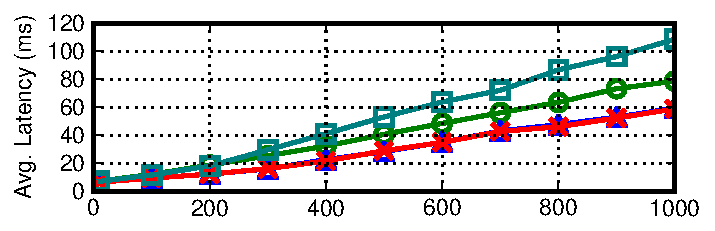
\includegraphics[width=\figscale\columnwidth]{figs/finals/2lan-threads-lats.pdf}
\vspace{-.5em}

\includegraphics[width=2.8in]{figs/hat-ycsb-label.pdf}
\begin{center}{A.) Within \texttt{us-east} \texttt{(VA)}}\end{center}
\end{center}
\begin{center}
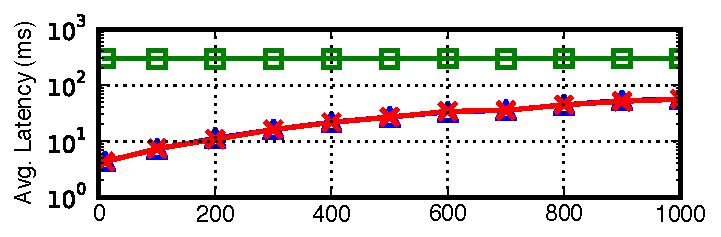
\includegraphics[width=\figscale\columnwidth]{figs/finals/2wan-threads-lats-log.pdf}\vspace{-.5em}

\includegraphics[width=2.8in]{figs/hat-ycsb-label.pdf}
\end{center}
\begin{center}{B.) Between \texttt{us-east} \texttt{(CA)} and 
    \texttt{us-west-2} \texttt{(OR)}}\end{center}\vspace{-.5em}
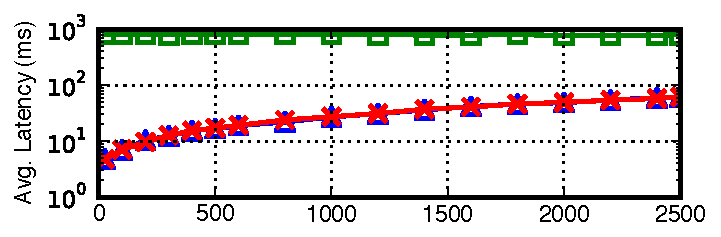
\includegraphics[width=\figscale\columnwidth]{figs/finals/5wan-threads-lats-log.pdf}\vspace{-.5em}

\includegraphics[width=2.8in]{figs/hat-ycsb-label.pdf}
\end{center}
\begin{center}{C.) Between \texttt{us-east} \texttt{(VA)}, \texttt{us-west-1} \texttt{(CA)},\\ \texttt{us-west-2} \texttt{(OR)}, \texttt{eu-west} \texttt{(IR)}, \texttt{ap-northeast} \texttt{(SI)}}\end{center}
\caption{YCSB latency for two clusters of five servers each 
  deployed within a single datacenter and cross-datacenters (note log
  scale for multi-datacenter deployment).}
\label{fig:wan-lat}
\end{figure}

\begin{figure}[t!]
\begin{center}

\includegraphics[width=.4\columnwidth]{figs/strategylegendthree.pdf}
\begin{center}{A.) Within \texttt{us-east} \texttt{(VA)}}\end{center}
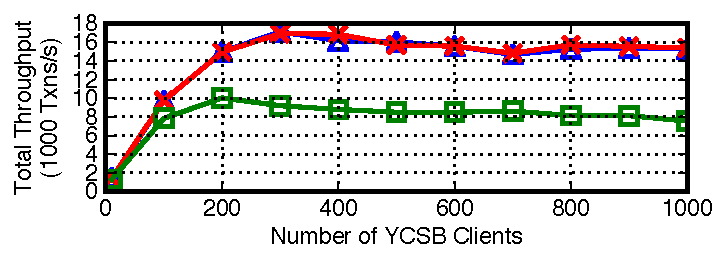
\includegraphics[width=\figscale\columnwidth]{figs/finals/2lan-threads-thru.pdf}
\begin{center}{B.) Between \texttt{us-east} \texttt{(CA)} and \texttt{us-west-2} \texttt{(OR)}}\end{center}
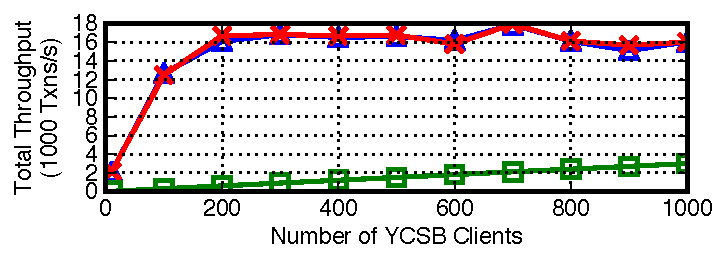
\includegraphics[width=\figscale\columnwidth]{figs/finals/2wan-threads-thru.pdf}
\begin{center}{C.) Between \texttt{us-east} \texttt{(VA)}, \texttt{us-west-1} \texttt{(CA)},\\ \texttt{us-west-2} \texttt{(OR)}, \texttt{eu-west} \texttt{(IR)}, \texttt{ap-northeast} \texttt{(SI)}}\end{center}
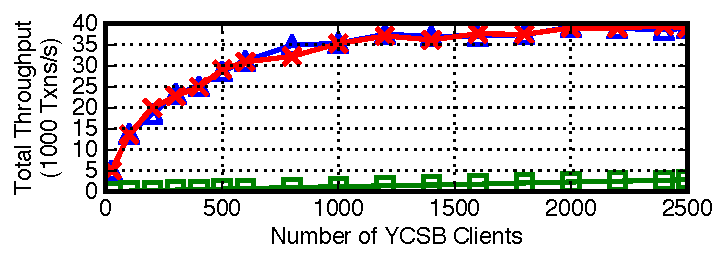
\includegraphics[width=\figscale\columnwidth]{figs/finals/5wan-threads-thru.pdf}
\end{center}
\caption{YCSB throughput for two clusters of five servers each 
  deployed within a single datacenter and cross-datacenters.}
\label{fig:wan-thru}
\end{figure}

\vspace{.5em}\noindent\textit{Geo-replication.} We first deploy the
database prototype across an increasing number of
datacenters. Figures~\ref{fig:wan-lat}A and~\ref{fig:wan-thru}A shows
that, when operating two clusters within a single datacenter,
mastering each data item results in approximately half the throughput
and double the latency of \texttt{eventual}. This is because
coordination-free models are able to utilize replicas in both clusters
instead of always contacting the (single)
master. \texttt{RC}---essentially \texttt{eventual} with
buffering---is almost identical to \texttt{eventual}. Latency
increases linearly with the number of YCSB clients.

In contrast, when the two clusters are deployed across the continental
United States (Figures~\ref{fig:wan-lat}B and~\ref{fig:wan-thru}B), the average latency of
\texttt{master} increases to $300$ms (a $278$--$4257\%$ latency
increase; average $37$ms latency per operation). For the same number
of YCSB client threads, \texttt{master} has substantially lower
throughput than the coordination-free configurations. Increasing the number of YCSB
clients \textit{does} increase the throughput of \texttt{master}, but
our Thrift-based server-side connection processing did not gracefully
handle more than several thousand concurrent connections. In contrast,
across two datacenters, the performance of eventual and RC are
near identical to a single-datacenter deployment.

\FloatBarrier

When five clusters (as opposed to two, as before) are deployed across
the five EC2 datacenters with lowest communication cost
(Figures~\ref{fig:wan-lat}C and~\ref{fig:wan-thru}C), the trend continues: \texttt{master}
latency increases to nearly $800$ms per transaction. As an attempt at
reducing this overhead, we implemented and benchmarked a variant of
quorum-based replication as in Dynamo~\cite{dynamo}, in which clients
sent requests to all replicas, which completed as soon as a majority
of servers responded (guaranteeing regular
semantics~\cite{herlihy-art}). This strategy (not pictured) did not
substantially improve performance due to the network topology and
because worst-case server load was unaffected.

Because \texttt{master} performed {far} better than our
textbook implementation, we have omitted performance data for
two-phase locking. In addition to incurring the same WAN round-trip
latency, locking also incurred substantial overheads due to mutual
exclusion. While techniques such as those recently proposed in
Calvin~\cite{calvin} can reduce the overhead of serializable
transactions by avoiding locking, our mastered implementation and the
data from Section~\ref{sec:latency} are reasonable lower bounds on
latency.

\begin{figure}[t!]
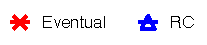
\includegraphics[width=.33\columnwidth]{figs/strategylegendtwo.pdf}\vspace{-1.5em}
\begin{center}
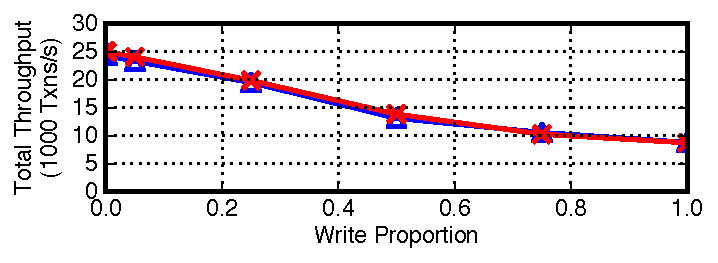
\includegraphics[width=\figscale\columnwidth]{figs/finals/wprop-thru.pdf}
\end{center}
\caption{Proportion of reads and writes versus throughput.}
\label{fig:rprop}
\begin{center}
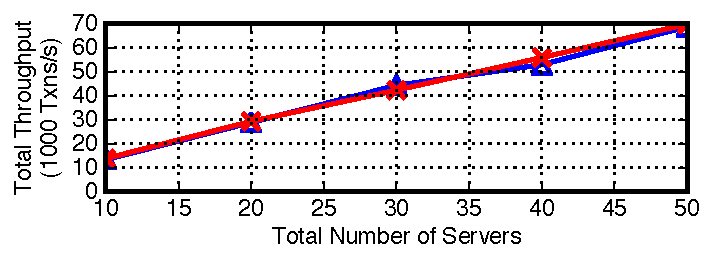
\includegraphics[width=\figscale\columnwidth]{figs/finals/scaleout-thru.pdf}
%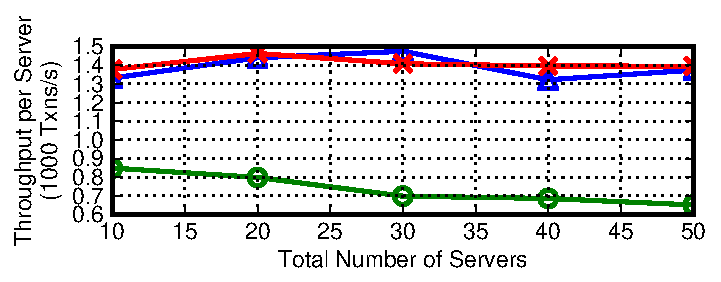
\includegraphics[width=\figscale\columnwidth]{figs/finals/scaleout-thru-perserver.pdf}
\end{center}
\caption{Scale-out of Eventual and RC.}
\label{fig:scaleout}
\end{figure}

\vspace{.5em}\noindent\textit{Read proportion.} Our default (equal)
proportion of reads and writes is fairly pessimistic: for example,
Facebook reports $99.8\%$ reads for their workload~\cite{eiger}. As
Figure~\ref{fig:rprop} demonstrates, increasing the proportion of
reads increases throughput; this is due to the decreased cost of read
operations on each node, and \texttt{RC} and \texttt{eventual} stay
matched in terms of throughput.

\vspace{.5em}\noindent\textit{Scale-out.} One of the key benefits of
our coordination-free algorithms is that they are shared-nothing~\cite{stonebraker-case}, meaning they
should not compromise scalability. Figure~\ref{fig:scaleout} shows
that varying the number of servers across two clusters in Virginia and
Oregon (with $15$ YCSB clients per server) results in linear scale-out
for \texttt{eventual} and \texttt{RC}. \texttt{RC} and
\texttt{eventual} scale linearly: increasing the number of servers per
cluster from $5$ to $25$ yields an approximately $5$x throughput
increase.

\vspace{.5em}\noindent\textit{Summary.} Our experimental prototype
confirms our earlier analytical intuition. Coordination-free systems
can provide useful semantics without substantial performance
penalties. Our coordination-free algorithms circumvent high WAN
latencies inevitable with non-coordination-free implementations. Our
results highlight Deutsch's observation that ignoring factors such as
latency can ``cause big trouble and painful learning
experiences''~\cite{fallacies-deutsch}---in a single-site context,
paying the cost of coordination may be tenable, but, especially as
services are geo-replicated, costs increase. In the next chapter, we
examine a more sophisticated set of implementations.

\FloatBarrier

\section{Isolation Models}
\label{sec:hat-definitions}

In this section, we formally define coordination-free transactional
semantics as a reference for the previous section. Our formalism is
based on that of Adya~\cite{adya}. For the reader familiar with his
formalism, this is a mostly-straightforward exercise combining
transactional models with distributed systems semantics. While the
novel aspects of this work largely pertain to \textit{using} these
definitions, we believe it is instructive to accompany them by
appropriate definitions as well.

To begin, we describe our model of weakly isolated transactions. This
is, with the exception of sessions, identical to that of
Adya~\cite{adya}. We omit a full duplication of his formalism here but
highlight several salient criteria. We refer the interested reader to
Adya's Ph.D. thesis, Section 3.1 (pp. 33--43).

Users submit transactions to a database system that contains a set of
objects, each of which is represented by multiple distinct
versions. Each transaction is composed of writes, which create new
versions of an object, and reads, which return a written version or
the initial version of the object. A transaction's last operation is
either \texttt{commit} or \texttt{abort}, and hence there is exactly one
invocation of either these two operations per
transaction. Transactions can either read individual items or read
based on predicates (or logical ``ranges'')      of data items.

\begin{definition}[Version set of a predicate-based operation]
When a transaction executes a read or write based on a predicate P,
the system selects a version for each tuple in P’s relations. The set
of selected versions is called the \textit{Version set} of this predicate-based
operation and is denoted by Vset(P).
\end{definition}

A history over transactions has two parts: first, a partial order of
events, comprised of several different types of edges that we describe
below, reflects the ordering of operations with respect to each
transaction, and, second, a order ($\ll$) on the committed versions of
each object. The history forms a graph, with nodes corresponding to
either transactions or operations within a transaction, and edges
constructed as we describe below.

As a departure from Adya's formalism, to capture the use of session
guarantees, we allow transactions to be grouped into sessions. We
represent sessions as a partial ordering on committed transactions
such that each transaction in the history appears in at most one
session.

\subsubsection{Framework}

To reason about isolation anomalies, we use Adya's concept of a
conflict graph, which is composed of dependencies between
transaction. The definitions in this section are directly from Adya,
with two differences. First, we expand Adya's formalism to deal
with \textit{per-item} dependencies. Second, we define session
dependencies (Definition~\ref{def:sd1}).

\begin{definition}[Change the Matches of a Predicate-Based Read]
A transaction $T_i$ changes the matches
of a predicate-based read $r_j$(P:Vset(P)) if $T_i$ installs $x_i$, $x_h$
immediately precedes $x_i$ in the version order, and $x_h$ matches
P whereas $x_i$ does not or vice-versa. In this case, we also
say that $x_i$ changes the matches of the predicate-based read.
The above definition identifies $T_i$ to be a transaction where
a change occurs for the matched set of $r_j$ (P: Vset(P)).
\end{definition}

\begin{definition}[Directly item-read-depends by $x$]
$T_j$ directly item-read-depends on transaction $T_i$ if $T_i$ installs some
  object version $x_i$ and $T_j$ reads $x_i$.
\end{definition}

\begin{definition}[Directly item-read-depends]
$T_j$ directly item-read-depends on transaction $T_i$ if $T_j$
  directly item-read-depends by $x$ on $T_i$ for some data item $x$.
\end{definition}

\begin{definition}[Directly predicate-read-depends by $P$]
Transaction $T_j$ directly predicate-read-depends by $P$ on
transaction $T_i$ if $T_j$ performs an operation $r_j$(P: Vset(P)),
$x_k$ $\in$ Vset(P), $i = k$ or $x_i \ll x_k$ , and $x_i$ changes the
matches of $r_j$ (P: Vset(P)).
\end{definition}


\begin{definition}[Directly Read-Depends{~\cite[Definition 2]{adya}}]
$T_j$ directly read-depends on transaction $T_i$ if it directly
item-read-depends or directly predicate-read-depends on $T_i$.
\end{definition}

\begin{definition}[Directly predicate-read-depends]
$T_j$ directly predicate-read-depends on $T_i$ if $T_j$ directly
  predicate-read-depends by $P$ on $T_i$ for some predicate $P$.
\end{definition}


\begin{definition}[Directly item-anti-depends by $x$]
$T_j$ directly item-anti-depends by $x$ on transaction $T_i$ if $T_i$
  reads some object version $x_k$ and $T_j$ installs $x$'s next
  version (after $x_k$) in the version order. Note that the
  transaction that wrote the later version directly item-anti-depends
  on the transaction that read the earlier version.
\end{definition}

\begin{definition}[Directly item-anti-depends]
$T_j$ directly item-anti-depends on transaction $T_i$ if $T_j$
  directly item-anti-depends on transaction $T_i$.
\end{definition}

\begin{definition}[Directly predicate-anti-depends by $P$]
$T_j$ directly predicate-anti-depends by $P$ on transaction $T_i$ if
  $T_j$ overwrites an operation $r_i(P:$ Vset(P)). That is, if $T_j$
  installs a later version of some object that changes the matches of
  a predicate based read performed by $T_i$.
\end{definition}

\begin{definition}[Directly Anti-Depends{~\cite[Definition 4]{adya}}]
Transaction $T_j$ directly anti-depends on transaction $T_i$ if it
directly item-anti-depends or directly predicate-anti-depends on
$T_i$.
\end{definition}

\begin{definition}[Directly Write-Depends by $x$]
A transaction $T_j$ directly write-depends by $x$ on transaction $T_i$
if $T_i$ installs a version $x_i$ and $T_j$ installs $x$'s next
version (after $x_i$) in the version order.
\end{definition}

\begin{definition}[Directly Write-Depends{~\cite[Definition 5]{adya}}]
A transaction $T_j$ directly write-depends on transaction $T_i$ if
$T_i$ directly write-depends by $x$ on $T_j$ for some item $x$.
\end{definition}

\begin{definition}[Session-Depends]
\label{def:sd1}
A transaction $T_j$ session-depends on transaction $T_i$ if $T_i$ and
$T_j$ occur in the same session and $T_i$ precedes $T_j$ in the
session commit order.
\end{definition}

The dependencies for a history $H$ form a graph called its Directed
Serialization Graph ($DSG(H)$). If $T_j$ directly write-depends on
$T_i$ by $x$, we draw $T_i\overset{ww_x}\longrightarrow T_j$. If $T_j$
read-depends on $T_i$ by $x$, we draw
$T_i \overset{wr_x}\longrightarrow T_j$. If $T_j$ directly
anti-depends on transaction $T_j$ by $x$, we draw
$T_i \overset{rw_x}\DashedArrow T_j$. If $T_j$ session-depends on
$T_i$ in session $S$, we draw $T_i \overset{S}\longrightarrow
T_j$~\cite[Definition 8]{adya}.

We also consider the Unfolded Serialization Graph ($USG(H)$) that is a
variation of the $DSG$. The USG is specified for the transaction of
interest, $T_i$, and a history, $H$, and is denoted by $USG(H,
T_i)$. For the USG, we retain all nodes and edges of the $DSG$ except
for $T_i$ and the edges incident on it. Instead, we split the node for
$T_i$ into multiple nodes---one node for every read/write event in
$T_i$. The edges are now incident on the corresponding operation of of
$T_i$.

$USG(H, T_i)$ is obtained by transforming $DSG(H)$ as follows:.  For
each node $p$ ($p \neq T_i$) in $DSG(H)$, we add a node to
$USG(H,T_i)$. For each edge from node $p$ to node $q$ in $DSG(H)$,
where p and q are different from $T_i$, we draw a corresponding edge
in $USG(H,T_i)$. Now we add a node corresponding to every read and
write performed by $T_i$. Any edge that was incident on $T_i$ in the
$DSG$ is now incident on the corresponding read or write operation on
$T_i$ in the $USG$. Finally, consecutive events in $T_i$ are connected
by \textit{order edges}, e.g., if an action (e.g., SQL statement)
reads object $y_j$ and immediately follows a write on object $x$ in
transaction $T_i$, we add an order-edge from $w_i(x_i)$ to
$r_i(y_j)$~\cite[Section 4.2.1]{adya}. Note that creating a graph
with ``supernodes'' replacing each set of read and write operations
for each $T_i$ in $USG(H)$ yields $DSG(H)$.

\subsubsection{Transactional Anomalies and Isolation Levels}
\label{sec:anomalies-hat}

Following Adya, we define isolation levels according to
possible \textit{anomalies}--typically represented by cycles in the
serialization graphs. Definitions~\ref{def:imp}--\ref{def:lostupdate}
are not found in Adya but are found (albeit not in this formalism) in
Berenson et al.~\cite{ansicritique} and the literature on session
guarantees~\cite{sessionguarantees, vogels-defs}.

\begin{definition}[Write Cycles (G0)]
A history $H$ exhibits phenomenon G0 if $DSG(H)$ contains a directed
cycle consisting entirely of write-dependency edges.
\end{definition}

\begin{definition}[Read Uncommitted]
A system that provides Read Uncommitted isolation prohibits phenomenon G0.
\end{definition}

\begin{definition}[Aborted Reads (G1a)]
A history $H$ exhibits phenomenon G1a if it contains an aborted
transaction $T_1$ and a committed transaction $T_2$ such that $T_2$ has read
some object (possibly via a predicate) modified by $T_1$.
\end{definition}

\begin{definition}[Intermediate Reads (G1b)]
  A history $H$ exhibits phenomenon G1b if it contains a committed
  transaction $T_2$ that has read a version of object $x$ (possibly
  via a predicate) written by transaction $T_1$ that was not $T_1$'s
  final modification of $x$.
\end{definition}

\begin{definition}[Circular Information Flow (G1c)]
A history $H$ exhibits phenomenon G1c if $DSG(H)$ contains a directed
cycle consisting entirely of dependency edges.
\end{definition}

\begin{definition}[Read Committed]
A system that provides Read Committed isolation prohibits phenomenon G0, G1a, G1b, and G1c.
\end{definition}

\begin{definition}[Item-Many-Preceders (IMP)]
\label{def:imp}
A history $H$ exhibits phenomenon IMP if $DSG(H)$ contains a
transaction $T_i$ such that $T_i$ directly item-read-depends by $x$ on more
than one other transaction.
\end{definition}

\begin{figure}[H]
\begin{align*}
\small
T_1 &: w_x(1)\\
T_2 &: w_x(2)\\
T_3 &: r_x(1)~r_x(2)
\end{align*}
\caption{Example of \textit{IMP} anomaly.}
\label{fig:nici-history}
\end{figure}

\begin{figure}[H]
\centering
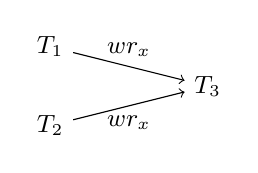
\begin{tikzpicture}[node distance=3cm]
\tikzstyle{tx}=[draw=none, fill=none]
\node[tx] (T1) at (0,0) {$T_1$};
\node[tx] (T2) at (0,-1) {$T_2$};
\node[tx] (T3) at (2,-.5) {$T_3$};

\draw[->] (T1) edge node[above]{$wr_x$} (T3);
\draw[->] (T2) edge node[below]{$wr_x$} (T3);
\end{tikzpicture}
\caption{DSG for Figure~\ref{fig:nici-history}.}
\label{fig:nici-dsg}
\end{figure}

\begin{definition}[Item Cut Isolation (I-CI)]
A system that provides Item Cut Isolation prohibits phenomenon IMP.
\end{definition}

\begin{definition}[Predicate-Many-Preceders (PMP)]
A history $H$ exhibits phenomenon PMP if, for all predicate-based
reads $r_i(P_i:Vset(P_i))$ and $r_j(P_j:Vset(P_j)$ in $T_k$ such that
the logical ranges of $P_i$ and $P_j$ overlap (call it $P_o$), the set
of transactions that change the matches of $P_o$ for $r_i$ and $r_j$
differ.
\end{definition}

\begin{definition}[Predicate Cut Isolation (P-CI)]
A system that provides Predicate Cut Isolation prohibits phenomenon PMP.
\end{definition}

\begin{definition}[Observed Transaction Vanishes (OTV)]
\label{def:otv}
A history $H$ exhibits phenomenon OTV if $USG(H)$ contains a directed
cycle consisting of exactly one read-dependency edge by $x$ from $T_j$
to $T_i$ and a set of edges by $y$ containing at least one
anti-dependency edge from $T_i$ to $T_j$ and $T_j$'s read from $y$
precedes its read from $x$.
\end{definition}
\begin{figure}[H]
\begin{align*}
\small
T_1 &: w_x(1)~w_y(1)\\
T_2 &: w_x(2)~w_y(2)\\
T_3 &: r_x(2)~r_y(1)
\end{align*}
\caption{Example of \textit{OTV} anomaly.}
\label{fig:nta-history}
\end{figure}

\begin{figure}[H]
\centering
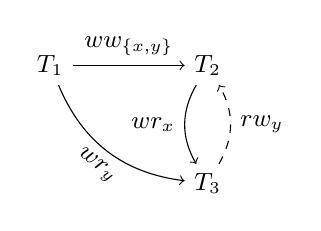
\begin{tikzpicture}[node distance=3cm]
\tikzstyle{tx}=[draw=none, fill=none]
\node[tx] (T1) at (0,0) {$T_1$};
\node[tx] (T2) at (2,0) {$T_2$};
\node[tx] (T3) at (2,-1.5) {$T_3$};

\draw[->] (T1) edge node[sloped, above]{$ww_{\{x, y\}}$} (T2);
\draw[->] (T1) edge [bend right] node[sloped, below]{$wr_y$} (T3);
\draw[->] (T2) edge [bend right] node[left]{$wr_x$} (T3);
\draw[dashed, ->] (T3) edge [bend right] node[right]{$rw_y$} (T2);
\end{tikzpicture}
\caption{DSG for Figure~\ref{fig:nta-history}.}
\label{fig:nta-dsg}
\end{figure}

\begin{definition}[Monotonic Atomic View (MAV)]
A system that provides Monotonic Atomic View isolation prohibits
phenomenon OTV in addition to providing Read Committed isolation.
\end{definition}

The following session guarantees are directly adapted from Terry et
al.'s original definitions~\cite{sessionguarantees}:

\begin{definition}[Non-monotonic Reads (N-MR)]
A history $H$ exhibits phenomenon N-MR if $DSG(H)$ contains a directed cycle
consisting of a transitive session-dependency between transactions
$T_j$ and $T_i$ with an anti-dependency edge by $i$ from $T_j$ and a
read-dependency edge by $i$ into $T_i$.
\end{definition}

\begin{definition}[Monotonic Reads (MR)]
A system provides Monotonic Reads if it prohibits phenomenon N-MR.
\end{definition}


\begin{figure}[H]
\begin{align*}
\small
T_1 &: w_x(1)\\
T_2 &: w_x(2)\\
T_3 &: r_x(2)\\
T_4 &: r_x(1)
\end{align*}
\caption{Example of \textit{N-MR} violation when $w_x(1) \ll w_x(2)$ and $T_4$ directly session-depends on $T_3$.}
\label{fig:nmr-history}
\end{figure}

\begin{figure}[H]
\centering
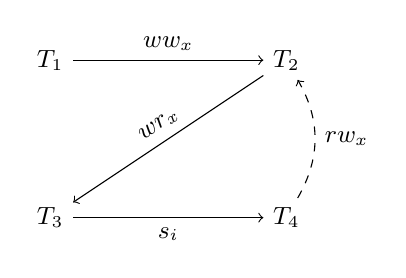
\begin{tikzpicture}[node distance=3cm]
\tikzstyle{tx}=[draw=none, fill=none]
\node[tx] (T1) at (0,0) {$T_1$};
\node[tx] (T2) at (3,0) {$T_2$};

\node[tx] (T3) at (0,-2) {$T_3$};
\node[tx] (T4) at (3,-2) {$T_4$};

\draw[->] (T1) edge node[above]{$ww_x$} (T2);
\draw[->] (T3) edge node[below]{$s_i$} (T4);

\draw[->] (T2) edge node[sloped, above]{$wr_x$} (T3);
%\draw[->] (T2) edge [bend right] node[left]{$wr_x$} (T4);
%\draw[->] (T1) edge [bend right]node[right]{$wr_x$} (T4);
\draw[dashed, ->] (T4) edge [bend right]node[right]{$rw_x$} (T2);
\end{tikzpicture}
\caption{DSG for Figure~\ref{fig:nmr-history}. $wr_x$ dependency from $T_1$ to $T_4$ omitted.} 
\label{fig:nmr-dsg}
\end{figure}

\begin{definition}[Non-monotonic Writes (N-MW)]
A history $H$ exhibits phenomenon N-MW if $DSG(H)$ contains a directed cycle
consisting of a transitive session-dependency between transactions
$T_j$ and $T_i$ and at least one write-dependency edge.
\end{definition}


\begin{figure}[H]
\begin{align*}
\small
T_1 &: w_x(1)\\
T_2 &: w_y(1)\\
T_3 &: r_y(1)~r_x(0)
\end{align*}
\caption{Example of \textit{N-MW} anomaly if $T_2$ directly session-depends on $T_1$.}
\label{fig:nmw-history}
\end{figure}

\begin{figure}[H]
\centering
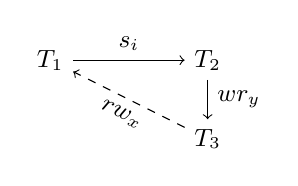
\begin{tikzpicture}[node distance=3cm]
\tikzstyle{tx}=[draw=none, fill=none]
\node[tx] (T1) at (0,0) {$T_1$};
\node[tx] (T2) at (2,0) {$T_2$};
\node[tx] (T3) at (2,-1) {$T_3$};

\draw[->] (T1) edge node[above]{$s_i$} (T2);
\draw[->] (T2) edge node[right]{$wr_y$} (T3);
\draw[->, dashed] (T3) edge node[below, sloped]{$rw_x$} (T1);
\end{tikzpicture}
\caption{DSG for Figure~\ref{fig:nmw-history}.}
\label{fig:nmw-dsg}
\end{figure}


\begin{definition}[Monotonic Writes (MW)]
A system provides Monotonic Writes if it prohibits phenomenon N-MW.
\end{definition}

\begin{definition}[Missing Read-Write Dependency (MRWD)]
A history $H$ exhibits phenomenon MRWD if, in $DSG(H)$, for all
committed transactions $T_1$, $T_2$, $T_3$ such that $T_2$
read-depends on $T_1$ and $T_3$ read-depends on $T_2$, $T_3$ does
not directly anti-depend on $T_1$.
\end{definition}


\begin{figure}[H]
\begin{align*}
\small
T_1 &: w_x(1)\\
T_2 &: r_x(1)~w_y(1)\\
T_3 &: r_y(1)~r_x(0)
\end{align*}
\caption{Example of \textit{MRWD} anomaly.}
\label{fig:nwfr-history}
\end{figure}

\begin{figure}[H]
\centering
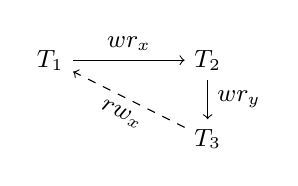
\begin{tikzpicture}[node distance=3cm]
\tikzstyle{tx}=[draw=none, fill=none]
\node[tx] (T1) at (0,0) {$T_1$};
\node[tx] (T2) at (2,0) {$T_2$};
\node[tx] (T3) at (2,-1) {$T_3$};

\draw[->] (T1) edge node[above]{$wr_x$} (T2);
\draw[->] (T2) edge node[right]{$wr_y$} (T3);
\draw[->, dashed] (T3) edge node[below, sloped]{$rw_x$} (T1);
\end{tikzpicture}
\caption{DSG for Figure~\ref{fig:nwfr-history}.}
\label{fig:nwfr-dsg}
\end{figure}

\begin{definition}[Writes Follow Reads (WFR)]
A system provides Writes Follow Reads if it prohibits phenomenon MWRD.
\end{definition}

\begin{definition}[Missing Your Writes (MYR)]
A history $H$ exhibits phenomenon MYR if $DSG(H)$ contains a directed cycle
consisting of a transitive session-dependency between transactions
$T_j$ and $T_i$, at least one anti-dependency edge, and the remainder
anti-dependency or write-dependency edges.
\end{definition}


\begin{figure}[H]
\begin{align*}
\small
T_1 &: w_x(1)\\
T_2 &: r_x(0)\\
\end{align*}
\caption{Example of \textit{MYR} anomaly if $T_2$ directly session-depends on $T_1$.}
\label{fig:nryw-history}
\end{figure}

\begin{figure}[H]
\centering
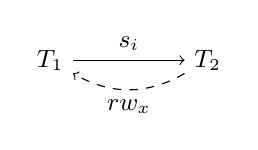
\begin{tikzpicture}[node distance=3cm]
\tikzstyle{tx}=[draw=none, fill=none]
\node[tx] (T1) at (0,0) {$T_1$};
\node[tx] (T2) at (2,0) {$T_2$};

\draw[->] (T1) edge node[above]{$s_i$} (T2);
\draw[dashed, ->] (T2) edge [bend left] node[below]{$rw_x$} (T1);
\end{tikzpicture}
\caption{DSG for Figure~\ref{fig:nwfr-history}.}
\label{fig:nryw-dsg}
\end{figure}

\begin{definition}[Read Your Writes (RYW)]
A system provides Read Your Writes if it prohibits phenomenon MYR.
\end{definition}

\begin{definition}[PRAM Consistency]
A system provides PRAM Consistency if it prohibits phenomenon N-MR,
N-MW, and MYR.
\end{definition}

\begin{definition}[Causal Consistency]
A system provides Causal Consistency if it provides PRAM Consistency
and prohibits phenomenon MWRD.
\end{definition}

\begin{definition}[Lost Update]
A history $H$ exhibits phenomenon Lost if $DSG(H)$ contains a directed
cycle having one or more item-antidependency edges and all edges are
by the same data item $x$.
\label{def:lostupdate}
\end{definition}

\begin{definition}[Write Skew (Adya G2-item)]
A history $H$ exhibits phenomenon Write Skew if $DSG(H)$ contains a directed
cycle having one or more item-antidependency edges.
\end{definition}

For Snapshot Isolation, we depart from Adya's recency-based definition
(see Adya Section 4.3). Nonetheless, implementations of this
definition will still be unavailable due to reliance of preventing
Lost Update.

\begin{definition}[Snapshot Isolation]
A system that provides Snapshot Isolation prevents phenomena G0, G1a,
G1b, G1c, PMP, OTV, and Lost Update.
\end{definition}

For Repeatable Read, we return to Adya.

\begin{definition}[Repeatable Read]
A system that provides Repeatable Read Isolation prohibits phenomena
G0, G1a, G1b, G1c, and Write Skew.
\end{definition}

\section{Summary}
\label{sec:conclusion}

In this chapter, we have shown that many previously defined isolation
and data consistency models from the database and distributed systems
communities are \iconfluent and can be implemented in a
coordination-free manner. While traditional implementations of several
of these semantics employ coordination, for those that we prove
\iconfluent, this is not strictly necessary. Thus, existing
applications that are built using one of these existing models may
enjoy the benefits of coordination-free execution.
